%%%%%%%% ICML 2025 EXAMPLE LATEX SUBMISSION FILE %%%%%%%%%%%%%%%%%

\documentclass{article}

% Recommended, but optional, packages for figures and better typesetting:
\usepackage{microtype}
\usepackage{graphicx}
\usepackage{subfigure}
\usepackage{booktabs} % for professional tables

% hyperref makes hyperlinks in the resulting PDF.
% If your build breaks (sometimes temporarily if a hyperlink spans a page)
% please comment out the following usepackage line and replace
% \usepackage{icml2025} with \usepackage[nohyperref]{icml2025} above.
\usepackage{hyperref}


% Attempt to make hyperref and algorithmic work together better:
\newcommand{\theHalgorithm}{\arabic{algorithm}}

% Use the following line for the initial blind version submitted for review:
% \usepackage{icml2025}

% If accepted, instead use the following line for the camera-ready submission:
\usepackage[accepted]{icml2025}
% Not an ICML paper: replace the proceedings notice in the first-page footnote.
\makeatletter\renewcommand{\Notice@String}{Test-task report: reproduction of ALDA \citep{batra2024alda}, October 2026.}\makeatother

% For theorems and such
\usepackage{amsmath}
\usepackage{amssymb}
\usepackage{mathtools}
\usepackage{amsthm}

% if you use cleveref..
\usepackage[capitalize,noabbrev]{cleveref}

%%%%%%%%%%%%%%%%%%%%%%%%%%%%%%%%
% THEOREMS
%%%%%%%%%%%%%%%%%%%%%%%%%%%%%%%%
\theoremstyle{plain}
\newtheorem{theorem}{Theorem}[section]
\newtheorem{proposition}[theorem]{Proposition}
\newtheorem{lemma}[theorem]{Lemma}
\newtheorem{corollary}[theorem]{Corollary}
\theoremstyle{definition}
\newtheorem{definition}[theorem]{Definition}
\newtheorem{assumption}[theorem]{Assumption}
\theoremstyle{remark}
\newtheorem{remark}[theorem]{Remark}

% Todonotes is useful during development; simply uncomment the next line
%    and comment out the line below the next line to turn off comments
%\usepackage[disable,textsize=tiny]{todonotes}
\usepackage[textsize=tiny]{todonotes}


% The \icmltitle you define below is probably too long as a header.
% Therefore, a short form for the running title is supplied here:
\icmltitlerunning{Reproducing ALDA: Zero-Shot Generalization Without Data Augmentation}

\begin{document}

\twocolumn[
\icmltitle{Reproducing ALDA: Zero-Shot Generalization of Vision-Based RL \\
           Without Data Augmentation}

\begin{icmlauthorlist}
\icmlauthor{Oleg Zhukov}{ind}
\end{icmlauthorlist}

\icmlaffiliation{ind}{Independent}

\icmlcorrespondingauthor{Oleg Zhukov}{zhukovol3q@gmail.com}

\icmlkeywords{Reinforcement Learning, Disentanglement, Associative Memory, Generalization}

\vskip 0.3in
]

\printAffiliationsAndNotice{}

\begin{abstract}
We reimplement Associative Latent DisentAnglement (ALDA), which gives
Soft Actor-Critic a QLAE-style disentangled latent space whose
per-dimension codebooks act as an associative memory, and test whether it
generalizes zero-shot to visual distribution shifts without any data
augmentation. We train on DeepMind Control \emph{walker-walk} from pixels for
1M environment steps (2 seeds) and evaluate periodically on a color-shift
environment and on the Distracting Control Suite (easy: dynamic DAVIS
backgrounds, camera and color perturbations). The agent reaches a return of
$778$ on the training environment and retains $81\%$ of it under color shift
and $43\%$ under Distracting CS, with both OOD curves still rising at the end of
training. Reconstructions show that the latent model maps distracted frames
back to the training appearance. However, the size of this associative
correction does not predict the per-evaluation performance gap.
\end{abstract}

\section{Introduction}
\label{sec:intro}

Policies learned from pixels typically break when the visual appearance of the
scene changes. The dominant fix is data augmentation
\citep{yarats2021drqv2,hansen2021svea}: expose the agent to approximations of
the test-time variations during training. ALDA \citep{batra2024alda} uses no
augmentation. It learns a disentangled latent representation with latent
quantization \citep{hsu2023qlae} and interprets the quantized latent model as
an associative (Hopfield-like) memory: at test time, an out-of-distribution
(OOD) encoding is pulled to the nearest stored in-distribution value in every
latent dimension, so that a change in a task-irrelevant factor (e.g.,
background) ideally only perturbs a few latents, which are then snapped back.

This report describes a from-scratch, single-file implementation of SAC+ALDA
built on CleanRL's SAC \citep{huang2022cleanrl}, trains it on DeepMind Control
\citep{tassa2018dmc}, and evaluates zero-shot transfer to the Distracting
Control Suite \citep{stone2021dcs}. We ask one research question: \emph{does the
associative latent model actually act on OOD observations, and does the size of
its correction explain the performance drop?} (\cref{sec:rq}).

\section{Method}
\label{sec:method}

\paragraph{SAC.} The base learner is Soft Actor-Critic
\citep{haarnoja2018sac} with a tanh-Gaussian actor, two critics with
Polyak-averaged targets, and automatic entropy tuning.

\paragraph{Disentanglement (QLAE).} An encoder $f_\theta$ maps \emph{a single}
RGB frame to a continuous vector $z_{cont}\in\mathbb{R}^{n_z}$. Each dimension
$j$ owns a scalar codebook $v_j\in\mathbb{R}^{|V|}$, and a decoder $g_\phi$
reconstructs the frame from the quantized latent. Strong weight decay on
$f_\theta$ and $g_\phi$, together with the per-dimension quantization,
encourages disentanglement \citep{hsu2023qlae}.

\paragraph{Association.} ALDA replaces QLAE's hard $\arg\min$ with a modern
Hopfield retrieval \citep{ramsauer2020hopfield} per dimension:
\begin{equation}
  z_{d,j} = \textstyle\sum_k \mathrm{softmax}\big(-\beta\,|z_{cont,j}-v_{jk}|\big)_k\, v_{jk}.
  \label{eq:assoc}
\end{equation}
With large $\beta$ this retrieves (almost) one stored value per dimension. The
codebook is \emph{not} pulled towards encoder outputs (no $\mathcal{L}_{quantize}$);
it is optimized only by the task (critic) loss, so the values act as
task-optimized memories the encoder must learn to map onto. The ALDA objective is
\begin{equation}
  \begin{aligned}
  \mathcal{L}_{ALDA} = {} & \|g_\phi(\tilde z) - o\|_2^2 + \|z_{cont} - \mathrm{sg}(z_d)\|_2^2 \\
  & + \lambda_\theta\|\theta\|^2 + \lambda_\phi\|\phi\|^2,
  \end{aligned}
\end{equation}
where $\tilde z = z_{cont} + \mathrm{sg}(z_d - z_{cont})$ is the
straight-through estimator.

\paragraph{Temporal information.} Frame stacks of $k{=}3$ are folded into the
batch, each frame is encoded and associated independently, and the $k$ latent
vectors are then combined by a small 1D CNN $h_\gamma$ over time
(\cref{alg:alda}). This keeps the autoencoder operating on single images,
which the original paper found necessary for disentanglement.

\begin{algorithm}[tb]
   \caption{SAC+ALDA update (one gradient step)}
   \label{alg:alda}
\begin{algorithmic}
   \STATE {\bfseries Input:} batch $(o, a, r, o', d)$, $o\in\mathbb{R}^{B\times 3k\times64\times64}$
   \STATE $x \leftarrow$ reshape $o$ to $Bk$ single frames
   \STATE $z_{cont} \leftarrow f_\theta(x)$; \ $z_d \leftarrow l_\psi(\mathrm{sg}(z_{cont}))$ \hfill (\cref{eq:assoc})
   \STATE $\mathcal{L}_{ALDA} \leftarrow \mathrm{MSE}(g_\phi(z_{cont}{+}\mathrm{sg}(z_d{-}z_{cont})), x) + \mathrm{MSE}(z_{cont}, \mathrm{sg}(z_d))$
   \STATE $h \leftarrow h_\gamma(\text{reshape } z_d \text{ to } B\times k\times n_z)$
   \STATE $y \leftarrow r + \gamma(1{-}d)\big(\min_i \bar Q_i(h', a') - \alpha\log\pi(a'|h')\big)$, $a'\sim\pi(\cdot|h')$
   \STATE $\mathcal{L}_Q \leftarrow \sum_i (Q_i(h,a) - y)^2$
   \STATE step $(\theta,\phi,\psi,\gamma,Q)$ on $\mathcal{L}_Q + \mathcal{L}_{ALDA}$ (AdamW)
   \IF{$t \bmod 2 = 0$}
   \STATE update $\pi$ and $\alpha$ on $\mathrm{sg}(h)$; Polyak-update $\bar Q, \bar h_\gamma$
   \ENDIF
\end{algorithmic}
\end{algorithm}

\section{Implementation}
\label{sec:impl}

The code is a single file (\texttt{alda.py}, ${\sim}570$ lines) with YAML
configs; all hyperparameters follow the paper's appendix table
(\cref{tab:hparams}).

\paragraph{Networks.} The encoder and decoder follow QLAE's appendix with
leaky ReLUs replaced by GELU, as in ALDA. \emph{Encoder:} 4 blocks of
[conv$3{\times}3$ s1, conv$3{\times}3$ s1, conv$4{\times}4$ s2] with widths
32/64/128/256, each conv followed by GELU and InstanceNorm ($64^2\!\to\!4^2$), then
two dense-256 ReLU layers and a linear map to $n_z{=}12$. \emph{Decoder:}
StyleGAN-like; $z$ goes through a 2-layer mapping MLP to a style vector $w$, a
learned $256{\times}4{\times}4$ input is upsampled by 12 transposed-conv layers
whose outputs are modulated by AdaIN from $w$, and a $1{\times}1$ conv outputs
RGB. \emph{Latent model:} $12{\times}12$ scalar codebooks, initialized to
$\mathrm{linspace}(-1,1)$, $\beta{=}100$. \emph{History encoder:} two Conv1d
layers (kernel 2, 64 channels, GELU) over the 3 per-frame latents. The critic
applies a linear projection to 50 features followed by two Q-MLPs
($2{\times}1024$, GELU); the actor has its own 50-d projection and a
$2{\times}1024$ tanh-Gaussian MLP.

\paragraph{Gradient routing.} We follow our reading of the paper's Fig.~2.
$\mathcal{L}_Q$ trains the Q-heads, the history encoder and the codebook
values, but stops at $z_{cont}$: the encoder receives gradients \emph{only}
from reconstruction and commitment. The actor uses the critic's history
encoder output with a stop-gradient, as in SAC+AE \citep{yarats2021sacae}.

\paragraph{Deviations and engineering choices.}
\textbf{(i) Decoupled weight decay.} With Adam and coupled L2 of $0.1$, the
weight-decay gradient swamped the reconstruction gradient and collapsed the
encoder to a constant output early in training. We therefore use AdamW
\citep{loshchilov2019adamw}, as in QLAE's own implementation, with decay
$0.1$ on the encoder and decoder only.
\textbf{(ii) Next-observation encoding.} Since frames are encoded
independently, $o'$ shares $k{-}1$ frames with $o$; we reuse their latents
and encode only the new frame for the TD target (exactly equivalent, ${\sim}2\times$
cheaper).
\textbf{(iii) Efficiency.} The replay buffer stores only the newest frame per
transition and rebuilds stacks at sampling time; the encoder/decoder run in
bf16 autocast (latent model, critic and actor stay in fp32); the scene is
rendered once per agent step instead of once per action repeat.
\textbf{(iv) Time limits} are treated as truncation and do not cut the
bootstrap.

\begin{table}[t]
\caption{Hyperparameters (identical for both seeds).}
\label{tab:hparams}
\vskip 0.1in
\begin{center}
\begin{small}
\begin{tabular}{lr}
\toprule
Parameter & Value \\
\midrule
Replay capacity / batch size & $10^6$ / 128 \\
Latent temperature $\beta$ & 100 \\
Latents $n_z$ / values per latent $|V|$ & 12 / 12 \\
Weight decay $\lambda_\theta=\lambda_\phi$ (AdamW) & 0.1 \\
Frame stack / action repeat & 3 / 4 \\
Observation & $9\times64\times64$ \\
Learning rate (all nets) / $\alpha$ lr & $10^{-3}$ / $10^{-4}$ \\
Initial temperature $\alpha$ & 0.1 \\
Actor / target update period & 2 / 2 \\
Polyak $\tau$ / discount $\gamma$ & 0.005 / 0.99 \\
Feature dim ($z_Q$, $z_\pi$) & 50 \\
Random-action warmup & 1000 agent steps \\
\bottomrule
\end{tabular}
\end{small}
\end{center}
\vskip -0.1in
\end{table}

\section{Experimental Setup}
\label{sec:setup}

\paragraph{Training.} We train on \emph{walker-walk} from $64{\times}64$ pixels
for $10^6$ environment steps ($2.5{\times}10^5$ agent steps, one gradient update
per agent step), with 2 seeds. Each run took roughly 9 hours on a single
RTX~3090, including evaluation. No augmentation is used at any point; the agent
only ever sees the standard DMC scene.

\paragraph{Zero-shot evaluation.} Every $10^4$ environment steps we run 5
deterministic episodes (tanh of the policy mean) in three environments, using
seeds disjoint from training:
\begin{itemize}
\item \textbf{Train}: the unmodified DMC task.
\item \textbf{Color shift}: the DCS color distraction with
  $\texttt{max\_delta}{=}0.5$ and no drift. Agent and floor RGB values are
  shifted by up to $\pm0.5$ once per episode. This is our stand-in for DMCGB
  ``color hard'' used in the paper; it is similar in spirit but not identical.
\item \textbf{Distracting CS (easy)}: dynamic DAVIS 2017 \citep{ponttuset2017davis}
  validation videos as background (4 videos), plus dynamic camera and color
  perturbations at scale 0.1 \citep{stone2021dcs}.
\end{itemize}
Besides returns, at every evaluation we log latent statistics over all frames
from the evaluation episodes: the mean associative shift
$|z_{cont}-z_d|$, the fraction of $z_{cont}$ entries outside their codebook's
range, the normalized entropy of codebook usage, and the reconstruction MSE
against the observed frame.

\section{Results}
\label{sec:results}

\begin{figure}[t]
\vskip 0.1in
\begin{center}
\centerline{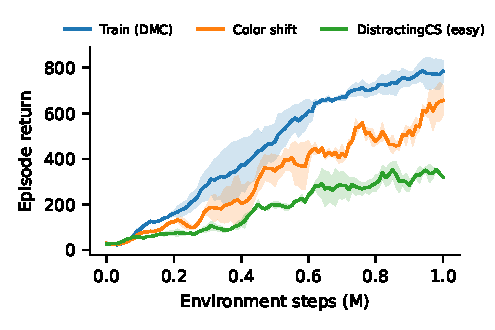
\includegraphics[width=\columnwidth]{figures/returns}}
\caption{Evaluation return on walker-walk vs.\ environment steps. Lines are
the mean over 2 seeds (moving average over 5 evaluations), shaded regions span
the two seeds. The OOD environments are never seen during training.}
\label{fig:returns}
\end{center}
\vskip -0.2in
\end{figure}

\begin{table}[t]
\caption{Evaluation return averaged over the last $10^5$ steps (11 evaluations
$\times$ 5 episodes). ``Retained'' is the ratio to the training-environment
return.}
\label{tab:returns}
\vskip 0.1in
\begin{center}
\begin{small}
\begin{tabular}{lcccc}
\toprule
Env & Seed 1 & Seed 2 & Mean & Retained \\
\midrule
Train          & 722 & 833 & 778 & 1.00 \\
Color shift    & 589 & 668 & 628 & 0.81 \\
DistractingCS  & 329 & 339 & 334 & 0.43 \\
\bottomrule
\end{tabular}
\end{small}
\end{center}
\vskip -0.1in
\end{table}

\paragraph{Learning curves.} \cref{fig:returns} and \cref{tab:returns}
summarize performance. On the training environment both seeds reach
700--850 return by 1M steps, and the curve is still rising. Zero-shot
performance appears in both OOD environments and keeps growing until the end
of training: the color-shift return climbs to ${\sim}630$ (81\% retained)
and Distracting CS to ${\sim}330$ (43\% retained), while a randomly initialized
agent scores ${\sim}30$ in all three. Variance is high in the OOD environments
(per-evaluation standard deviation across 5 episodes of 150--200 vs.\ 40--50 on
train): some episodes transfer almost perfectly while others fail, which fits
the per-episode sampling of distractors.

\begin{figure*}[t]
\vskip 0.1in
\begin{center}
\centerline{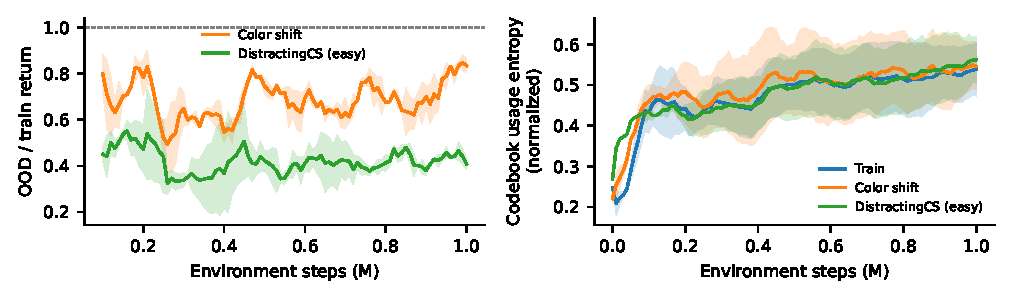
\includegraphics[width=\textwidth]{figures/retention_entropy}}
\caption{Left: OOD return as a fraction of the training-environment return
(from $10^5$ steps on, moving average over 5 evaluations; shaded: seed range).
Right: normalized entropy of codebook usage on evaluation frames from each
environment.}
\label{fig:retention}
\end{center}
\vskip -0.2in
\end{figure*}

\paragraph{Retention.} Dividing the OOD return by the training return
(\cref{fig:retention}, left) removes the effect of the agent getting better at
the task itself. Distracting CS retention is roughly flat at $0.35$--$0.5$ throughout training,
so the absolute DCS gains in \cref{fig:returns} mostly track improvement on the
training task. Color-shift retention dips to ${\sim}0.6$ between 0.3M and 0.8M
steps and recovers to ${\sim}0.85$ by 1M steps. Codebook usage entropy
(\cref{fig:retention}, right) rises over the first $2{\times}10^5$ steps and
then grows slowly. It is nearly identical on training and OOD frames, so OOD
inputs are spread over the stored values as broadly as training inputs.

\begin{figure}[t]
\vskip 0.1in
\begin{center}
\centerline{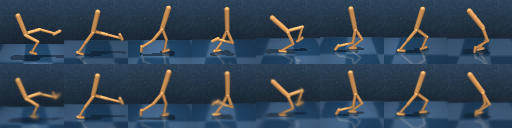
\includegraphics[width=\columnwidth]{figures/recon_train_s1}}
\vskip 0.03in
\centerline{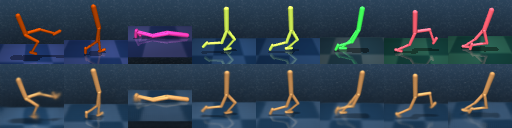
\includegraphics[width=\columnwidth]{figures/recon_color_s1}}
\vskip 0.03in
\centerline{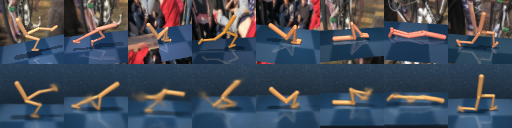
\includegraphics[width=\columnwidth]{figures/recon_dcs_s1}}
\caption{Inputs (top of each pair) and reconstructions $g_\phi(z_d)$ (bottom)
at 1M steps, seed 1. From top: train, color shift, Distracting CS. OOD
colors and DAVIS backgrounds are replaced by the training appearance
(orange walker, blue checkered floor) while the pose is largely kept.}
\label{fig:recon}
\end{center}
\vskip -0.2in
\end{figure}

\paragraph{Reconstructions.} \cref{fig:recon} shows the association step at
work. Under color shift, the
recolored walker (red, green, magenta) and tinted floors are decoded as the
canonical orange walker on the blue floor, with the correct pose. Under
Distracting CS, the DAVIS background (people, bicycles) is removed entirely;
the decoder renders the training floor and sky. The errors are in the pose.
Several DCS reconstructions show blurred or wrong limb configurations, likely
because the camera perturbation moves the walker
within the frame, which is a task-relevant change that the training data never
covered.

\begin{figure}[t]
\vskip 0.1in
\begin{center}
\centerline{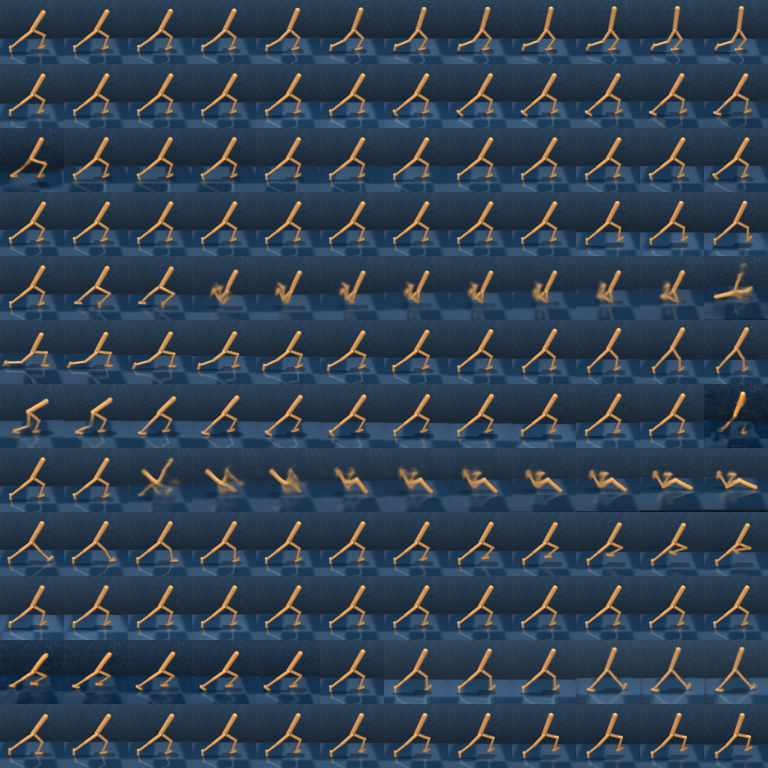
\includegraphics[width=0.9\columnwidth]{figures/traversal_s1}}
\caption{Latent traversals at 1M steps (seed 1). Row $i$ sweeps latent $i$
over its 12 sorted codebook values, with the others fixed at $z_d$ of a
training frame.}
\label{fig:traversal}
\end{center}
\vskip -0.2in
\end{figure}

\paragraph{Latent traversals.} \cref{fig:traversal} shows that individual latents
control interpretable aspects of the walker's configuration: some rows sweep
a single leg forward/backward, rows 5 and 8 move the torso from upright to
falling/lying, and others shift the body slightly in height or position.
Because the training scene never changes appearance, no latent encodes
background or color. This is expected, and it means OOD appearance can only be
handled by association, since there is no distractor latent to absorb it. The
latents are not perfectly disentangled: the torso latents also bend the legs.
Codebook usage entropy at the end of training is $0.60$ and $0.47$ of the
maximum (seed 1/2), i.e., most dimensions use only a subset of their 12 values.

\section{Research Question: Does Association Explain Generalization?}
\label{sec:rq}

\begin{figure*}[t]
\vskip 0.1in
\begin{center}
\centerline{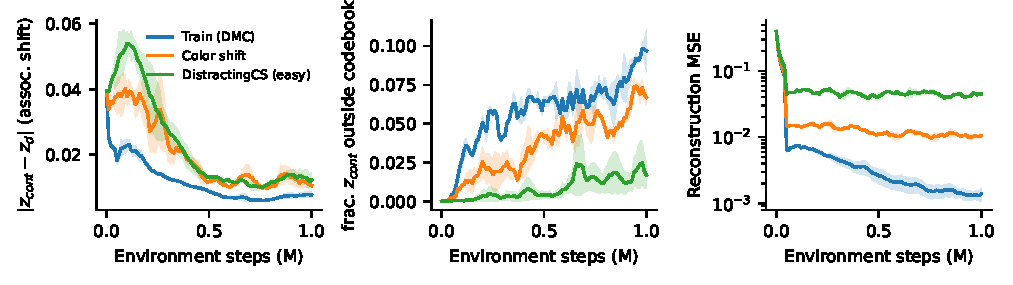
\includegraphics[width=\textwidth]{figures/latent_stats}}
\caption{Latent statistics on evaluation frames over training (mean over 2
seeds, shaded: seed range). Left: mean associative shift $|z_{cont}-z_d|$.
Middle: fraction of encoder outputs outside the range of their codebook.
Right: reconstruction MSE of $g_\phi(z_d)$ against the observed (possibly
distracted) frame, log scale.}
\label{fig:latent}
\end{center}
\vskip -0.2in
\end{figure*}

ALDA's central claim is that the latent model ``remaps'' OOD latents to
in-distribution values. We ask two things: (a) is the associative correction
measurably larger on OOD frames? (b) does its magnitude track how much return
is lost?

\paragraph{(a) Association acts more on OOD frames.} After the first
$2{\times}10^5$ steps, the mean shift $|z_{cont}-z_d|$ is on average $1.73\times$
larger on color-shift frames and $1.80\times$ larger on DCS frames than on
training frames (\cref{fig:latent}, left). Early in training, while the
encoder has not yet committed to the codebook, all three are high and the OOD
shift is ${\sim}2$--$3\times$ the train shift. OOD encodings do
\emph{not} fall outside the codebook range more often (\cref{fig:latent},
middle). On training frames ${\sim}9$--$10\%$ of encoder outputs lie beyond the
extreme codebook values (the encoder ``overshoots'' and is clipped by
association), but only ${\sim}1$--$3\%$ do on DCS. OOD inputs therefore land
\emph{between} stored values, where a soft Hopfield retrieval with
$\beta{=}100$ has to pick one of two neighbours and can pick the wrong one. The
reconstruction error against the distracted frame
(\cref{fig:latent}, right) is $10\times$ (color) and $30\times$ (DCS) the
training error and stays flat over training, consistent with the distractor
being projected out instead of reconstructed (\cref{fig:recon}).

\begin{figure*}[t]
\vskip 0.1in
\begin{center}
\centerline{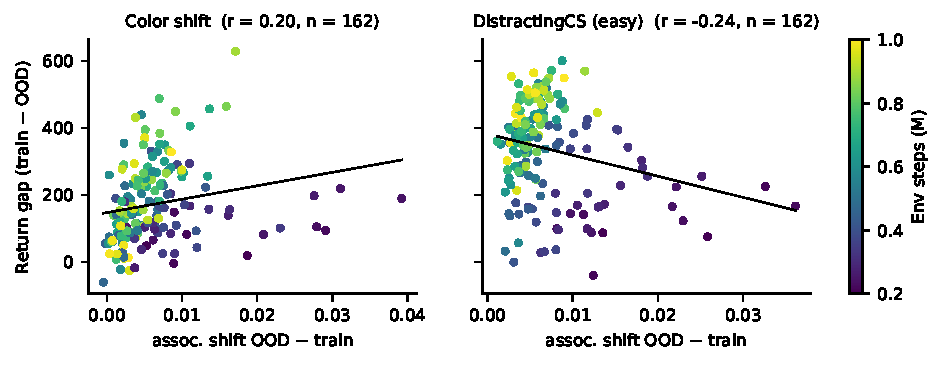
\includegraphics[width=0.85\textwidth]{figures/rq_scatter}}
\caption{Per-evaluation associative shift (OOD minus train) vs.\ return gap
(train minus OOD), both seeds, evaluations after $2{\times}10^5$ steps. Color
encodes training progress; the line is a least-squares fit.}
\label{fig:rq}
\end{center}
\vskip -0.2in
\end{figure*}

\paragraph{(b) The size of the correction does not predict the loss.} Pooling
all evaluations after $2{\times}10^5$ steps (81 per seed, $n{=}162$), the
Pearson correlation between the OOD-minus-train associative shift and the
train-minus-OOD return gap is $0.20$ for color shift and $-0.24$ for DCS.
Both are weak, and they have opposite signs. Over training the shift
\emph{decreases} (left panel) while the return gap \emph{increases} in absolute
terms (\cref{fig:returns}). The average magnitude of association is a
poor proxy for whether it helps. \cref{fig:rq} shows that what little
correlation there is comes from training progress: early evaluations (dark)
have a large shift and a small gap because returns are still low
everywhere. Within the late, bright points there is no visible trend.

\paragraph{Answer.} Yes, the associative latent model acts more strongly on OOD
observations. Qualitatively it does what ALDA claims: distractor appearance is
mapped back to the training appearance. The amount it moves the latents does
not predict performance. Our guess is that performance depends on whether the
retrieved values keep the task-relevant factors (pose) intact: the DCS failures
in \cref{fig:recon} are pose errors, and the background never leaks into the
reconstruction. A more
targeted diagnostic would measure retrieval errors in the latents that
encode task-relevant factors, which requires ground-truth state labels for
the evaluation frames. We leave this to future work.

\section{Limitations and Open Items}
\label{sec:limits}

\begin{itemize}
\item \textbf{Scope.} Only walker-walk with 2 seeds was trained to 1M steps.
  Configs for cartpole-balance, ball\_in\_cup-catch and finger-spin exist and
  pass short smoke tests, but were not run to completion. The paper uses 5
  seeds and 4 tasks.
\item \textbf{No baselines.} We did not train SAC+AE, SVEA or a
  SAC+QLAE ablation under the same budget, so we cannot attribute the
  OOD returns to association specifically. The ablation that removes
  \cref{eq:assoc} (hard quantization) is the most informative next experiment.
\item \textbf{Environments.} Our color shift is the DCS color wrapper, not the
  DMCGB ``color hard'' environment, and we evaluate DCS only at the easy level.
\item \textbf{Ambiguities.} The paper's table lists Adam; we use AdamW for the
  encoder/decoder (\cref{sec:impl}). The exact gradient routing and the
  history-encoder architecture are inferred from the paper's Fig.~2 and may
  differ from the authors' code.
\end{itemize}

\section{Conclusion}

Our single-file SAC+ALDA learns walker-walk from pixels and, without
any augmentation, transfers zero-shot to unseen color shifts (81\% of training
return) and partly to the Distracting Control Suite (43\%). Both OOD curves
keep improving with training. Reconstructions show that the associative
latent model maps distracted observations back to the training appearance.
Its average correction magnitude, however, does not explain the residual
performance gap, which appears to come from task-relevant (pose) errors under
camera shift.

\section*{Software and Data}

Code, configs and the plotting script for this report are available at
\url{https://github.com/zxclwnq/test-alda}. Training:
\texttt{python alda.py configs/walker\_walk.yaml seed=1}. Figures:
\texttt{python report/plots.py} and \texttt{python report/plots\_extra.py}.

\section*{Impact Statement}

This paper presents work whose goal is to advance the field of
Machine Learning. There are many potential societal consequences
of our work, none which we feel must be specifically highlighted here.

\bibliography{example_paper}
\bibliographystyle{icml2025}

%%%%%%%%%%%%%%%%%%%%%%%%%%%%%%%%%%%%%%%%%%%%%%%%%%%%%%%%%%%%%%%%%%%%%%%%%%%%%%%
% APPENDIX
%%%%%%%%%%%%%%%%%%%%%%%%%%%%%%%%%%%%%%%%%%%%%%%%%%%%%%%%%%%%%%%%%%%%%%%%%%%%%%%
\newpage
\appendix
\onecolumn
\section{Seed 2 Visualizations}

\begin{figure}[h]
\begin{center}
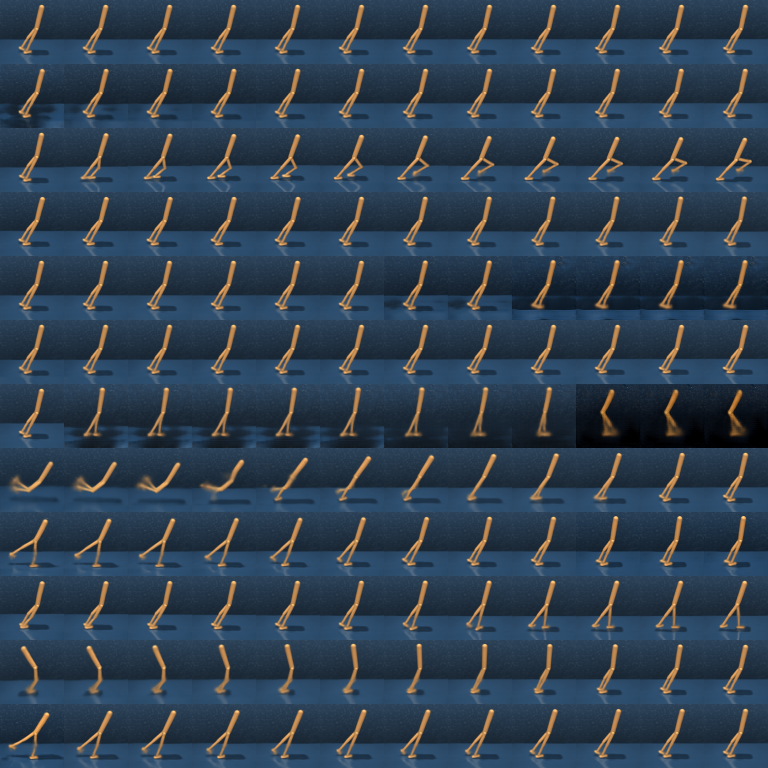
\includegraphics[width=0.48\textwidth]{figures/traversal_s2}
\hfill
\begin{minipage}[b]{0.48\textwidth}
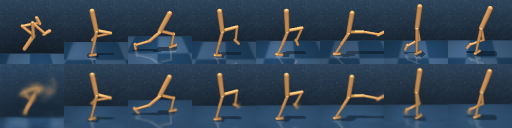
\includegraphics[width=\textwidth]{figures/recon_train_s2}\\[2pt]
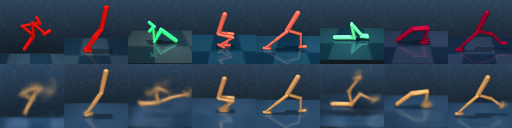
\includegraphics[width=\textwidth]{figures/recon_color_s2}\\[2pt]
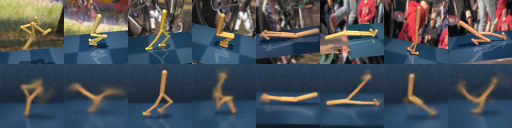
\includegraphics[width=\textwidth]{figures/recon_dcs_s2}
\end{minipage}
\caption{Seed 2 at 1M steps. Left: latent traversals (as in
\cref{fig:traversal}). Right: reconstructions on train, color shift and
Distracting CS (as in \cref{fig:recon}).}
\end{center}
\end{figure}

\section{Training Dynamics}

\begin{figure}[h]
\begin{center}
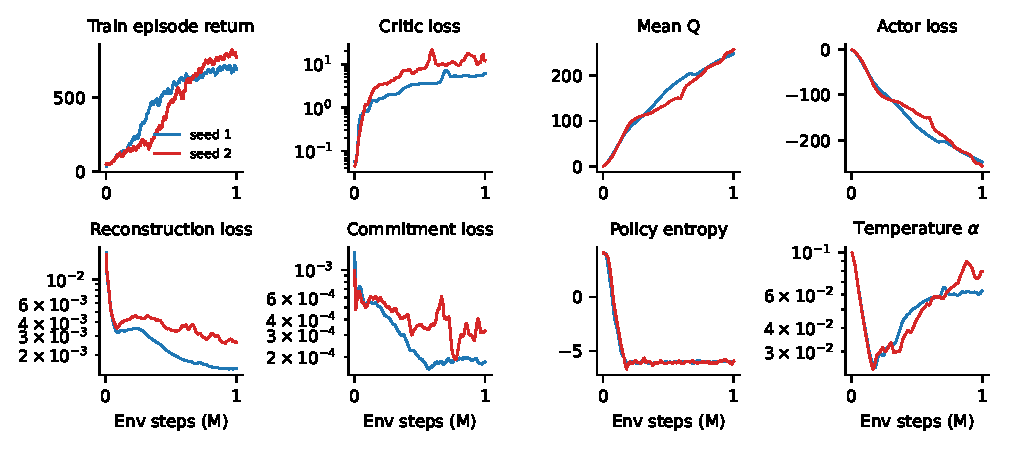
\includegraphics[width=\textwidth]{figures/training_dynamics}
\caption{Per-episode training statistics (losses averaged over the updates
within each episode, moving average over 20 episodes). Policy entropy
reaches the SAC target $-|\mathcal{A}|=-6$ within ${\sim}10^5$ steps, after which
$\alpha$ is adjusted to hold it there. Seed 2 has a ${\sim}2\times$ higher critic
loss and a higher reconstruction/commitment loss, but also the higher return.}
\label{fig:dynamics}
\end{center}
\end{figure}

Reconstruction and commitment losses drop by an order of magnitude within the
first $5{\times}10^4$ steps and then keep decreasing slowly
(\cref{fig:dynamics}). Commitment stays two orders of magnitude below
reconstruction, i.e., the encoder stays close to the codebook without an explicit
$\mathcal{L}_{quantize}$. Mean $Q$ grows smoothly and the critic loss never
diverges.

\section{Evolution of Reconstructions and Traversals}

\begin{figure}[h]
\begin{center}
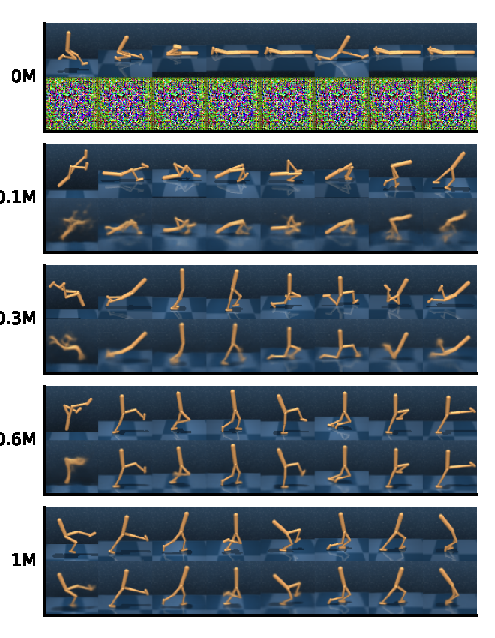
\includegraphics[width=0.32\textwidth]{figures/recon_train_evolution}
\hfill
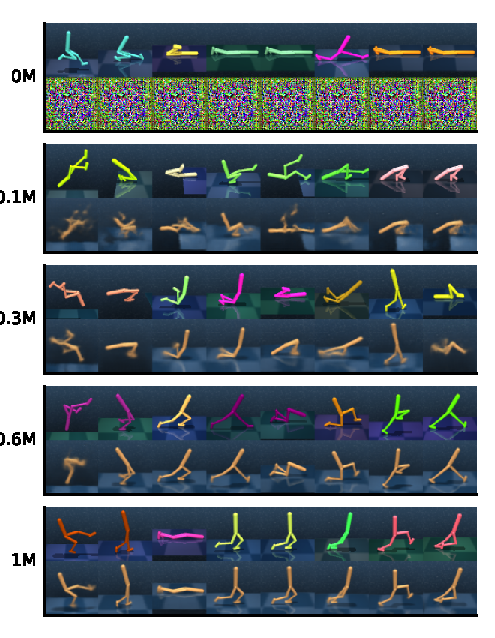
\includegraphics[width=0.32\textwidth]{figures/recon_color_evolution}
\hfill
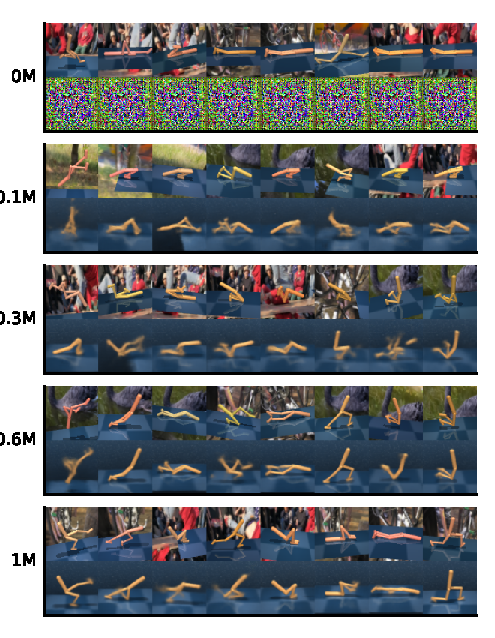
\includegraphics[width=0.32\textwidth]{figures/recon_dcs_evolution}
\caption{Inputs and reconstructions at 0, 0.1M, 0.3M, 0.6M and 1M steps (seed 1,
from the TensorBoard image log). Left to right: train, color shift, Distracting
CS. From 0.1M steps on, OOD backgrounds and colors are already decoded as the
training scene; later training mainly sharpens the walker's pose.}
\label{fig:recon-evo}
\end{center}
\end{figure}

\begin{figure}[h]
\begin{center}
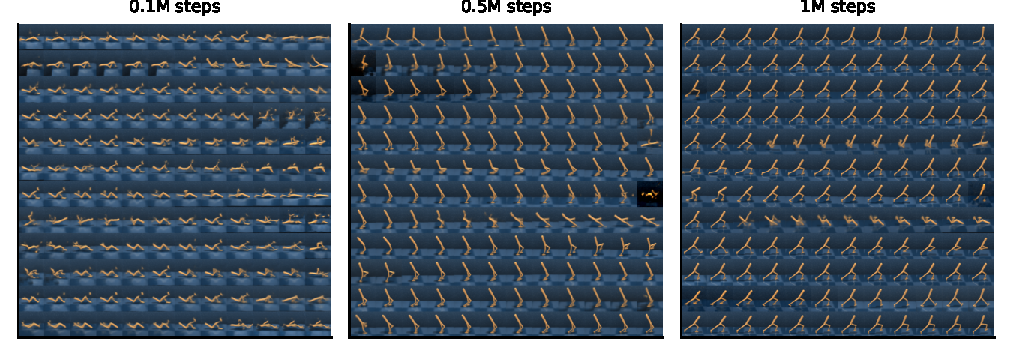
\includegraphics[width=\textwidth]{figures/traversal_evolution}
\caption{Latent traversals at 0.1M, 0.5M and 1M steps (seed 1). At 0.1M most
latents barely change the image; by 0.5M several latents control distinct
limb and torso configurations, and the traversals become smoother by 1M.}
\label{fig:trav-evo}
\end{center}
\end{figure}

\end{document}

% This document was modified from the file originally made available by
% Pat Langley and Andrea Danyluk for ICML-2K. This version was created
% by Iain Murray in 2018, and modified by Alexandre Bouchard in
% 2019 and 2021 and by Csaba Szepesvari, Gang Niu and Sivan Sabato in 2022.
% Modified again in 2023 and 2024 by Sivan Sabato and Jonathan Scarlett.
% Previous contributors include Dan Roy, Lise Getoor and Tobias
% Scheffer, which was slightly modified from the 2010 version by
% Thorsten Joachims & Johannes Fuernkranz, slightly modified from the
% 2009 version by Kiri Wagstaff and Sam Roweis's 2008 version, which is
% slightly modified from Prasad Tadepalli's 2007 version which is a
% lightly changed version of the previous year's version by Andrew
% Moore, which was in turn edited from those of Kristian Kersting and
% Codrina Lauth. Alex Smola contributed to the algorithmic style files.
